\documentclass[a4paper]{article}

\usepackage[pagebackref=false,colorlinks,urlcolor = blue,linkcolor=blue,citecolor=blue]{hyperref}

\usepackage{indentfirst}
\usepackage{amsmath,amsfonts,amssymb,amsthm}
\usepackage{geometry}
\usepackage{enumitem}
\usepackage{amsmath}
\usepackage[usenames,dvipsnames]{color,xcolor}
\definecolor{mygreen}{RGB}{28,172,0} % color values Red, Green, Blue
\definecolor{mylilas}{RGB}{170,55,241}
\usepackage{listings}
\usepackage{hyperref}
\hypersetup{linkcolor=blue}
\usepackage{graphicx}
\usepackage{emptypage}
\usepackage{afterpage}
\usepackage{titlesec}
\usepackage{wrapfig}
\usepackage{tikz}
\usetikzlibrary{arrows,decorations.markings}

\titleformat{\section}
{\normalfont\fontsize{20}{20}\bfseries}{\thesection}{1em}{}

\titleformat{\subsection}
{\normalfont\fontsize{15}{20}\bfseries}{\thesubsection}{1em}{}

\titleformat{\subsubsection}
{\normalfont\fontsize{12}{20}\bfseries}{\thesubsubsection}{1em}{}

\usepackage{pdfpages}
\usepackage{tikz}
\usepackage[american]{circuitikz}
\renewcommand{\baselinestretch}{1.2} 
\lstset{language=Matlab,%
	%basicstyle=\color{red},
	breaklines=true,%
	morekeywords={matlab2tikz},
	keywordstyle=\color{blue},%
	morekeywords=[2]{1}, keywordstyle=[2]{\color{black}},
	identifierstyle=\color{black},%
	stringstyle=\color{mylilas},
	commentstyle=\color{mygreen},%
	showstringspaces=false,%without this there will be a symbol in the places where there is a space
	numbers=left,%
	numberstyle={\tiny \color{black}},% size of the numbers
	numbersep=9pt, % this defines how far the numbers are from the text
	emph=[1]{for,end,break},emphstyle=[1]\color{blue}, %some words to emphasise
	%emph=[2]{word1,word2}, emphstyle=[2]{style},    
}

\geometry{
	a4paper,
	total={170mm,257mm},
	left=20mm,
	top=20mm,
}

\usepackage{xcolor}
\usepackage{listings}

\definecolor{mGreen}{rgb}{0,0.6,0}
\definecolor{mGray}{rgb}{0.5,0.5,0.5}
\definecolor{mPurple}{rgb}{0.58,0,0.82}
\definecolor{backgroundColour}{rgb}{0.95,0.95,0.92}


\lstdefinestyle{JavaStyle}{
	backgroundcolor=\color{backgroundColour},   
	commentstyle=\color{mGreen},
	keywordstyle=\color{magenta},
	numberstyle=\tiny\color{mGray},
	stringstyle=\color{mPurple},
	  basicstyle=\ttfamily\small,
	breakatwhitespace=false,         
	breaklines=true,                 
	captionpos=b,                    
	keepspaces=true,                 
	numbers=left,                    
	numbersep=5pt,                  
	showspaces=false,                
	showstringspaces=false,
	showtabs=false,                  
	tabsize=2,
	language=java
}



\usepackage{fancyhdr}
\pagestyle{fancy}
\fancyhf{}
\rhead{\textbf{Phase \#3}}
\lhead{\textbf{Advanced Programming Project}}
\cfoot{(\space \space \space \space \textbf{\thepage}  \space \space \space)}
\renewcommand{\headrulewidth}{1pt}
\renewcommand{\footrulewidth}{1pt}
\setlength{\parindent}{0ex}
\setlength{\parskip}{0ex}


%\usepackage{xepersian}
%\setlatintextfont[Scale=1]{Times New Roman}
%\settextfont{XB Niloofar}
%\setdigitfont{XB Niloofar}
%\DefaultMathsDigits 
%\makeatletter
%\bidi@patchcmd{\@Abjad}{آ}{الف}
%{\typeout{Succeeded in changing `آ` into `الف`}}
%{\typeout{Failed in changing `آ` into `الف`}}
%\makeatother
%\PersianAlphs

\DeclareMathOperator*{\epi}{\mathbf{epi}\space} 
\DeclareMathOperator*{\hypo}{\mathbf{hypo}\space} 
\DeclareMathOperator*{\dom}{\mathbf{dom}\space} 
\DeclareMathOperator*{\intt}{\mathbf{int}\space} 
\DeclareMathOperator*{\diag}{\mathbf{diag}\space} 
\DeclareMathOperator*{\minmz}{\mathrm{minimize}\:} 
\DeclareMathOperator*{\maxmz}{\mathrm{maximize}\:} 
\DeclareMathOperator*{\tr}{\mathrm{trace}} 
\DeclareMathOperator*{\st}{\mathrm{subject\:to}\:} 

\begin{document}
	
\begin{titlepage}
	
	\begin{center}
		\textbf{
			In The Name Of God\\
		}
		\vspace{2cm}
		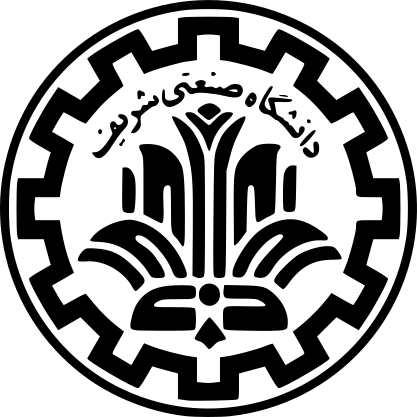
\includegraphics[scale=0.25]{logo.png}\\
		\vspace{0.5cm}
		\begin{Large}
			\textbf{
				Sharif University of Technology\\
				\vspace{0.5cm}
				Computer Science Department\\
			}
		\end{Large}
		\vspace{2.5cm}
		\begin{huge}
			\textbf{
				Advanced Programming Project\\
				 Phase 3\\
				\vspace{1cm}
				Hearthstone\\
			}
		\end{huge}
		\vspace{1.5cm}
		\begin{Large}
			\textbf{
				\\
				\vspace{1cm}
				Amirhossein Afsharrad\\
				\vspace{0.5cm}
				95101077\\
				\vspace{2cm}
				\today
			}
		\end{Large}
		
	\end{center}
	
	\thispagestyle{empty}
\end{titlepage}	

\large
\tableofcontents
\clearpage
\section{Introduction}
In this document we briefly explain the important points of the implementation of Hearthstone project's third phase. The goal for this phase is to complete the implementation of the game, so one can really play it. You may find all packages and classes attached to this report, or you can check them using the following link on GitHub:
\begin{center}
	\url{https://github.com/AmirAfsharrad/Hearthstone}
\end{center}
The java version of this project is java11 and it has been built using \textit{Gradle}. Apart from java standard packages, only the two following dependencies have been added to the \texttt{build.gradle} file for the \texttt{gson} and \texttt{json} respective packages:
\begin{itemize}
	\item \texttt{compile 'com.googlecode.json-simple:json-simple:1.1.1'}
	\item \texttt{compile group: 'com.google.code.gson', name: 'gson', version: '2.8.5'}
\end{itemize}
All the code has been generated by the author of this report, and no code has been copied from other resources. The resource for the images is also similar to the previous phase of the project.

\clearpage
\section{What has changed since phase 2?}
The most important advancement of the project is the full implementation of the game logic. Apart from that, there has been some changes made to the graphical user interface. These include the design of the second player on the playground panel, and some slight features such as progress bars for time and quests.

\clearpage
\section{The General Structure of the Game Logic}
Several elements have been added to the project in order to make the game logic work properly. These elements shall be explained in more detail later, but we are going to go through them in a short review here. First of all, the class \texttt{Contestant} has been added to the project to be responsible for each of the two players in the game. To be more clear, each player is actually a \texttt{Contestant} with some features and abilities. Using this class, any event that happens during the game for a player is reflected to this class and the proper choice of actions are made using the fields and methods of this class. The two contestants exist within the class \texttt{Playground}, which is a \texttt{Place} as described in previous reports.

Another useful structure lies within the package \texttt{GameLogic}, containing some \textit{visitor} classes responsible for acts such as dealing damage to game objects or restoring their health. Another important class inside this package is \texttt{PlayCards}, which is responsible for the procedure of having a card played.

To describe the big picture, game events are transferred from the game panel to the \texttt{Playground}, from which appropriate methods of \texttt{Contestant}s are called, and these methods usually include calling another method from \texttt{PlayCards} or different visitors of the package \texttt{GameLogic}.

These packages and classes are explained in more detail in next sections.

\clearpage
\section{The Class \texttt{Contestant}}
This class is the role model for each of the two players playing the game on the playground. There are several fields and methods withing this class, \textit{some} of which are explained below:
\subsection{fields}
There are many fields inside this class, each holding a game parameter for a player. These include name, mana, passive, hero, deck, hand, planted cards, the state of the player (which is either normal or waiting for target), current spell, current weapon, current quest, etc.

\subsection{Methods}
There are several methods in this class. Some with more importance are listed below:
\begin{itemize}
	\item 
	\texttt{public void init(Deck inputDeck)}\\
	This method does all the needed initialization for a player to start the game. There is a deck as the input to this method, which has been selected in the collections panel before starting the game. For the second player who does not select a deck, a default deck has been defined in the \texttt{GameHandler}, so that would be the input to this method in case.
	
	There are other methods used within \texttt{init}, including \texttt{initDeck}, \texttt{initHero}, \texttt{initHand}, and \texttt{initPassiveProcess}. The latter does what needs to be done in order to apply the effect of the passive selected by the user. Others methods are obvious by their names.
	
	\item \texttt{public void drawRandomCard(boolean noSpell)}\\
	This method, as expected from its name, draws a random card from deck to hand. It also has a boolean input which determines whether the drawn card can be a spell or not.
	
	\item \texttt{public void startTurn()}\\
	This method is responsible for starting a turn for a contestant. It handles whatever needs to be handled at the start of a turn, such as increasing the mana value (if it has not reached the maximum limit), or discarding some effects remaining from the previous turn of the opponent.
	
	\item \texttt{public void endTurn()}\\
	This method is similar to the previous one, but takes the appropriate actions when a player's turn finishes.
	
	\item \texttt{drawEffectHandle(Card card)}\\
	Some minions have effects which act at the time of drawing cards. For example, there are minions who would make any drawn cards have less cost than usual. This holds only when the minion is planted. There has been a structure defined to address these effects and this method checks these effects for all planted minions. If there is any, it takes the proper action.
	
	\item \texttt{private void startTurnMinionEffectHandle()}\\
	This method is similar to the previous one. The difference is about the time of action. While the previous method was responsible to take action about the effects of the planted minions at the time of card draw, this method does the same thing at the time of starting a turn.
	
	\item \texttt{private void startTurnWeaponEffectHandle()}\\
	This method does the same thing as the previous one, but for the weapons instead of minions.
	
	\item \texttt{private void endTurnMinionEffectHandle()}\\
	As described before, the function of this method is almost obvious. It handles the effects of the planted minions when a turn ends.
	
	\item \texttt{public void checkForDeadMinions()}\\
	This is a simple but very important and useful method for removing the dead minions from the game panel. Obviously, it is called several times from different places.
	
	\item \texttt{private void handleQuestCompletion(Card card)}\\
	This method is responsible to take proper actions when a user finishes a quest successfully. This includes giving the user the predefined reward.
	
	\item \texttt{public void runHeroPower()}\\
	This method is run whenever the user chooses to use the hero power of his or her hero. It handles the hero power effect based on the type of the hero.
	
	\item \texttt{public void initiateAttack(Attacker attacker, int attackValue)}\\
	This method initiates attack when the user decides to do so. The input is an \texttt{Attacker}, an interface implemented by minions and weapons. When a user clicks on a planted minion (and has not been waiting for a target to be received), it initiates an attack. It also can happen by clicking on the active weapon.
	
	\item \texttt{public void playCard(Card card, int numberOnLeft)}\\
	This method is responsible for playing a card when it is selected from the hand of the user. There is a class called \texttt{PlayCard}, whose methods are called within this method. Actually, this method could be removed and we could have used directly the \texttt{PlayCard} class methods, but we have avoided doing so for the sake of respecting the hierarchy. The class \texttt{PlayCards} is explained in the next section.
	
\end{itemize}

There are many more methods in this class, but they are not as important as the methods explained above. Many of those methods have been declared to do small jobs and do not need to be mentioned here.

\clearpage
\section{The Package \texttt{GameLogic}}
This package contains the classes added to the project in order to implement the game logic in a more structured manner. There are two packages and one class inside this package, which will be explained below.

\subsection{The Class \texttt{PlayCards}}
This class only contains four static methods listed below:
\begin{itemize}
	\item \texttt{public static void playSpell(Spell spell)}
	\item \texttt{public static void playMinion(Card card, int numberOnLeft)
	\item \texttt{public static void playWeapon(Weapon weapon)}}
	\item \texttt{public static void playQuest(Quest quest)}
\end{itemize}

	Obvious from their names, these methods are responsible for playing each of the four types of cards. While the methods for weapons and quests are quite small, the other two have many lines of codes since minions and spells are quite complicated to implement. Further explanations would be too detailed for this report, so we leave that part to the code itself. The only point to be made is about the battlecries of the minions, which have been implemented using the spells. Each battlecry is actually a spell, so we have defined new spell cards for each of the minions who have battlecries, and used this similarity to make our coding more convenient.
	
\subsection{The Package \texttt{Visitors}}
There are four visitor classes defined in this package:
\begin{itemize}
	\item \texttt{AttackVisitor}
	\item \texttt{DealDamageVisitor}
	\item \texttt{GiveHealthVisitor}
	\item \texttt{ModifyAttackVisitor}
\end{itemize}

These classes are used for attacking, dealing damage, giving (or restoring) health, and modifying the attack power of the game objects. They use the \textit{visitor} design pattern.

\subsection{The Package \texttt{Interfaces}}
This package contains the interfaces needed for the visitor classes to function properly. There interfaces are listed below:
\begin{itemize}
	\item \texttt{Attackable}
	\item \texttt{Attacker}
	\item \texttt{Damageable}
	\item \texttt{HealthTaker}
	\item \texttt{ModifiableAttack}
	\item \texttt{Target}
\end{itemize}
The functionality of these interfaces is known by their name. For instance, the \texttt{AttackVisitor} operates on \texttt{Attackable}, which is implemented by minions and heroes.

Having defined this structure, we have made the process of implementing the game logic much more convenient.








\end{document}






